\documentclass[aspectratio=169,10pt]{beamer}

\usetheme{metropolis}
\usepackage{appendixnumberbeamer}

\usepackage{booktabs}
\usepackage[scale=2]{ccicons}

\usepackage{pgfplots}
\usepgfplotslibrary{dateplot}

\usepackage{xspace}
\newcommand{\themename}{\textbf{\textsc{metropolis}}\xspace}

\usepackage{graphicx}
\usepackage{fontspec}
\usepackage{setspace}
\usepackage{listings}
\usepackage{amsmath}

% Uses Ethereum colorful logo instead of bullet, for all item levels.
\defbeamertemplate{itemize item}{image}{\large
\includegraphics[height=1.6ex]{images/bullet}}
\defbeamertemplate{itemize subitem}{image}{\large
\includegraphics[height=1.6ex]{images/bullet}}
\defbeamertemplate{itemize subsubitem}{image}{\large
\includegraphics[height=1.6ex]{images/bullet}}
\setbeamertemplate{itemize item}[image]
\setbeamertemplate{itemize subitem}[image]
\setbeamertemplate{itemize subsubitem}[image]


% Sets the template background image for all the slides.
% Change opacity here.
\setbeamertemplate{background}{%
	\begin{tikzpicture}[remember picture,overlay]
		\node[at=(current page.center),opacity=0.2]{
			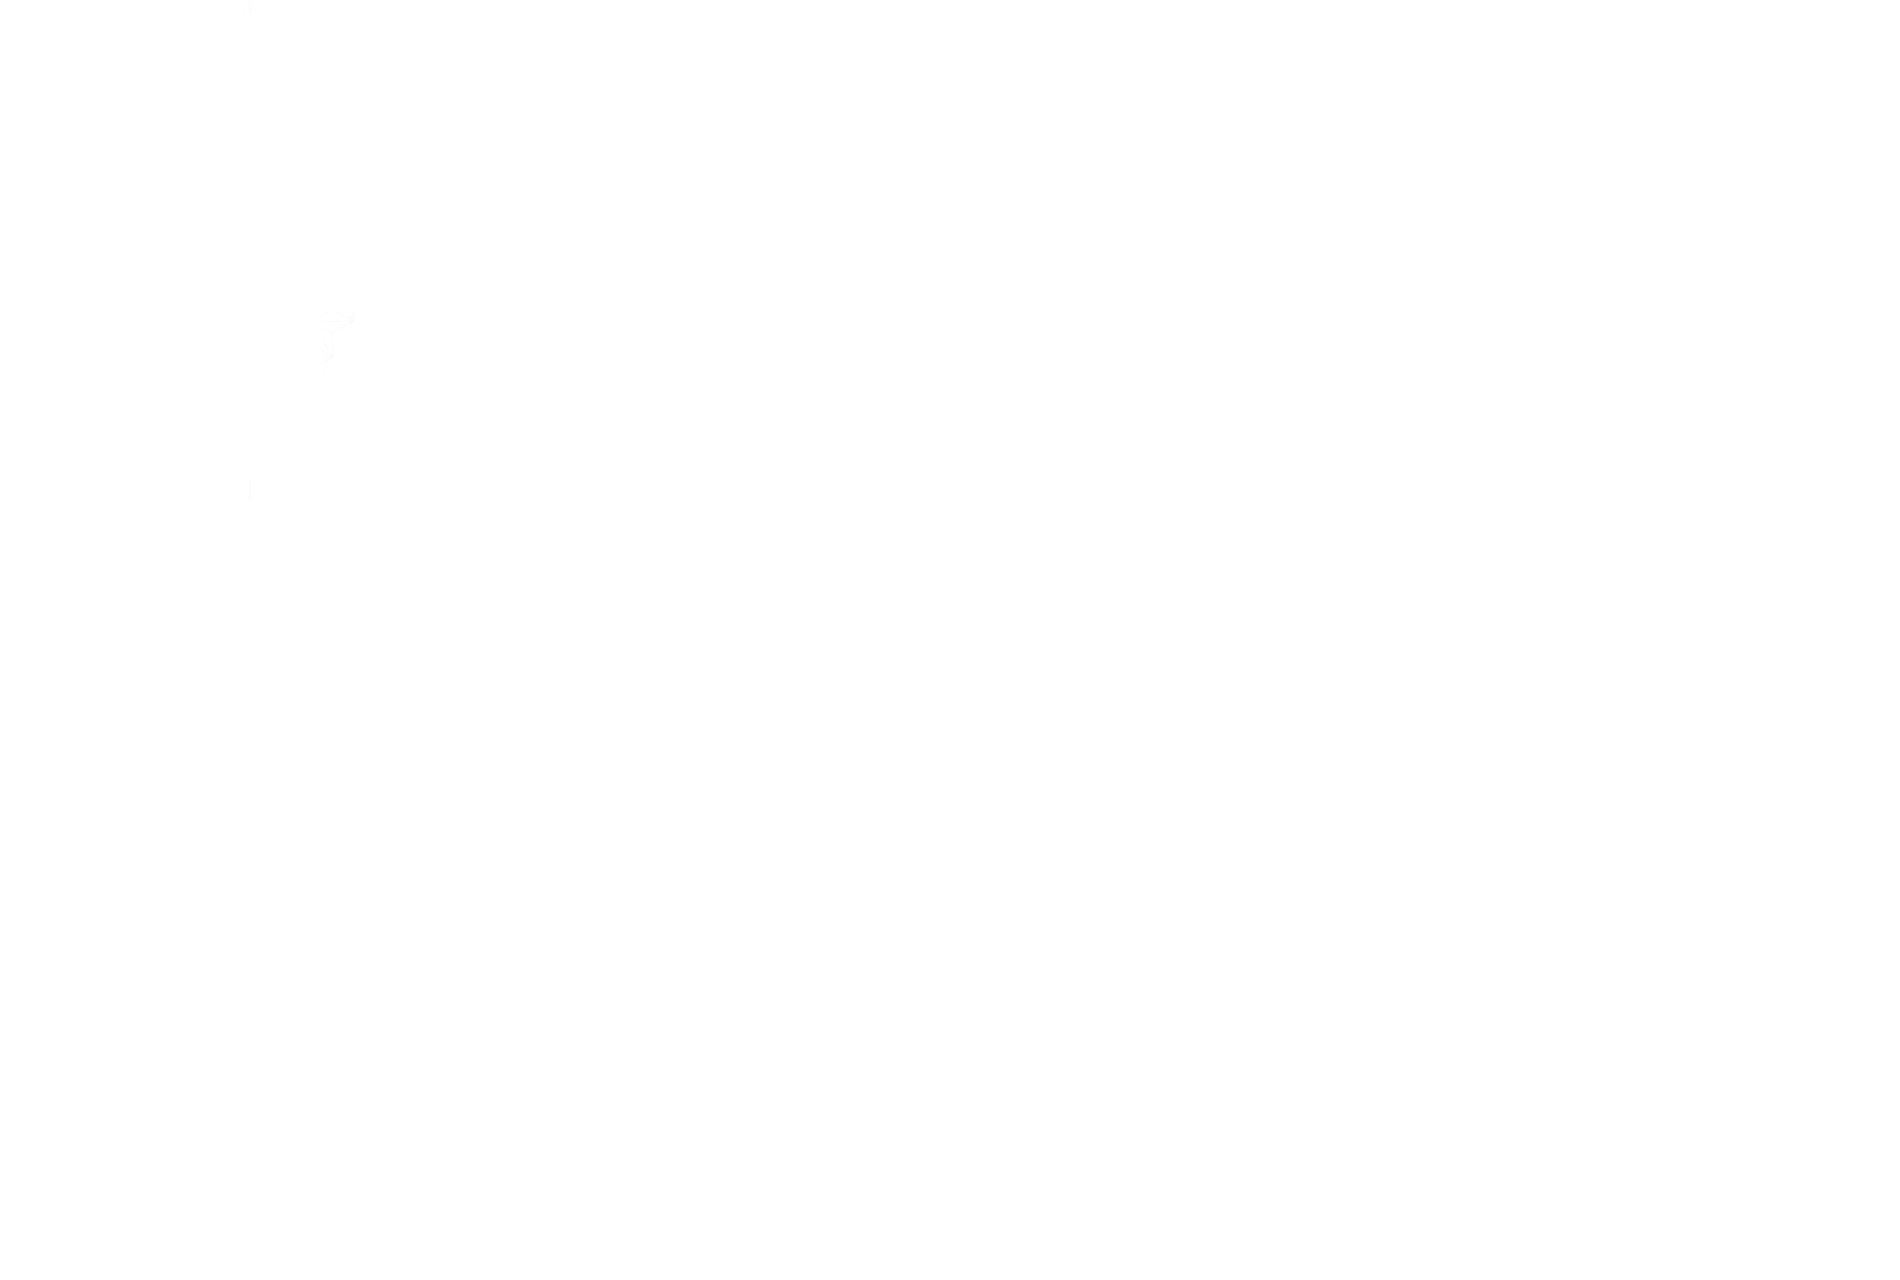
\includegraphics[width=\paperwidth,height=\paperheight]{images/bg}
		};
	\end{tikzpicture}
}


% Sets the color theme.
% Change here for light theme.
% `sectionpage=none` removes slide between sections.
%\metroset{background=dark,sectionpage=none}
%\metroset{background=light}
\metroset{background=dark}
\usebeamercolor[fg]{normal text}

% Sets the footer `devcon v` on the bottom right.
% Change `devcon v` text color here.
\setbeamercolor{frame footer}{fg=gray}
\setbeamertemplate{frame footer}{ethcc4 - github.com/leonardoalt/ethcc}

% Sets the new fonts.
\setsansfont{Circular Std Bold}
\setmonofont{Overpass Mono}

% Sets the default line spacing.
\setstretch{1.5}

% Sets monospace font for tables and quotes.
\AtBeginEnvironment{table}{\ttfamily}
\AtBeginEnvironment{quote}{\ttfamily}
\AtBeginEnvironment{figure}{\ttfamily}

% Sets the normal text font as monospace.
\setbeamerfont{normal text}{family=\ttfamily}
\AtBeginDocument{\usebeamerfont{normal text}}

% If you use the light theme, you need to manually change the
% icons to `_black`.
% Change your GitHub username here.
\setbeamertemplate{github}{
  \small
\includegraphics[height=1.6ex]{icons/github_white}
  \texttt{leonardoalt, MrChico}
}
% Change your email here.
\setbeamertemplate{email}{
  \small
\includegraphics[height=1.6ex]{icons/email_white}
  \texttt{\{leo, martin.lundfall\}@ethereum.org}
}
% Change your twitter account here.
\setbeamertemplate{twitter}{
  \small
\includegraphics[height=1.6ex]{icons/twitter_white}
  \texttt{leonardoalt, MartinLundfall}
}

% Remove here any contact you do not want to show.
\setbeamertemplate{contact}{
  \vspace*{2mm}
  \usebeamertemplate{github}\\
  \usebeamertemplate{email}\\
  \usebeamertemplate{twitter}
}

% Change presentation data here.
\title{{\huge Fully Automated Formal Verification:\\How far can we go?}}
\author{{\large Leo Alt \& Martin Lundfall}}
% Change date here.
% Empty date removes it from the frame.
% \date{\today} prints compilation date.
%Otherwise prints content.
\date{} %\date{\today}
\institute{{\large Ethereum Foundation}}
% Sets the Ethereum/devcon logo on the upper left.
\titlegraphic{\vfill
\includegraphics[height=1.2cm]{images/devcon}}

\lstdefinelanguage{Solidity}{
  keywords={break, continue, new, do, while, for, if, else, true, false, return, returns, msg, tx, block, this, require, assert, revert, throw},
  morecomment=[l]{//},
  morecomment=[s]{/*}{*/},
  morestring=[b]',
  morestring=[b]",
  ndkeywords={contract, import, pragma, bool, uint, public, internal, view, pure, payable, using, function},
  keywordstyle=\color{mLightBlue}\bfseries,
  ndkeywordstyle=\color{mLightRed}\bfseries,
  identifierstyle=\color{mAlmostWhite},
  commentstyle=\color{mLightPurple}\ttfamily,
  stringstyle=\color{mLightPink}\ttfamily,
  sensitive=true
}

\begin{document}

{
\setbeamertemplate{background}{%
	\begin{tikzpicture}[remember picture,overlay]
		\node[at=(current page.center),opacity=0.1]{
			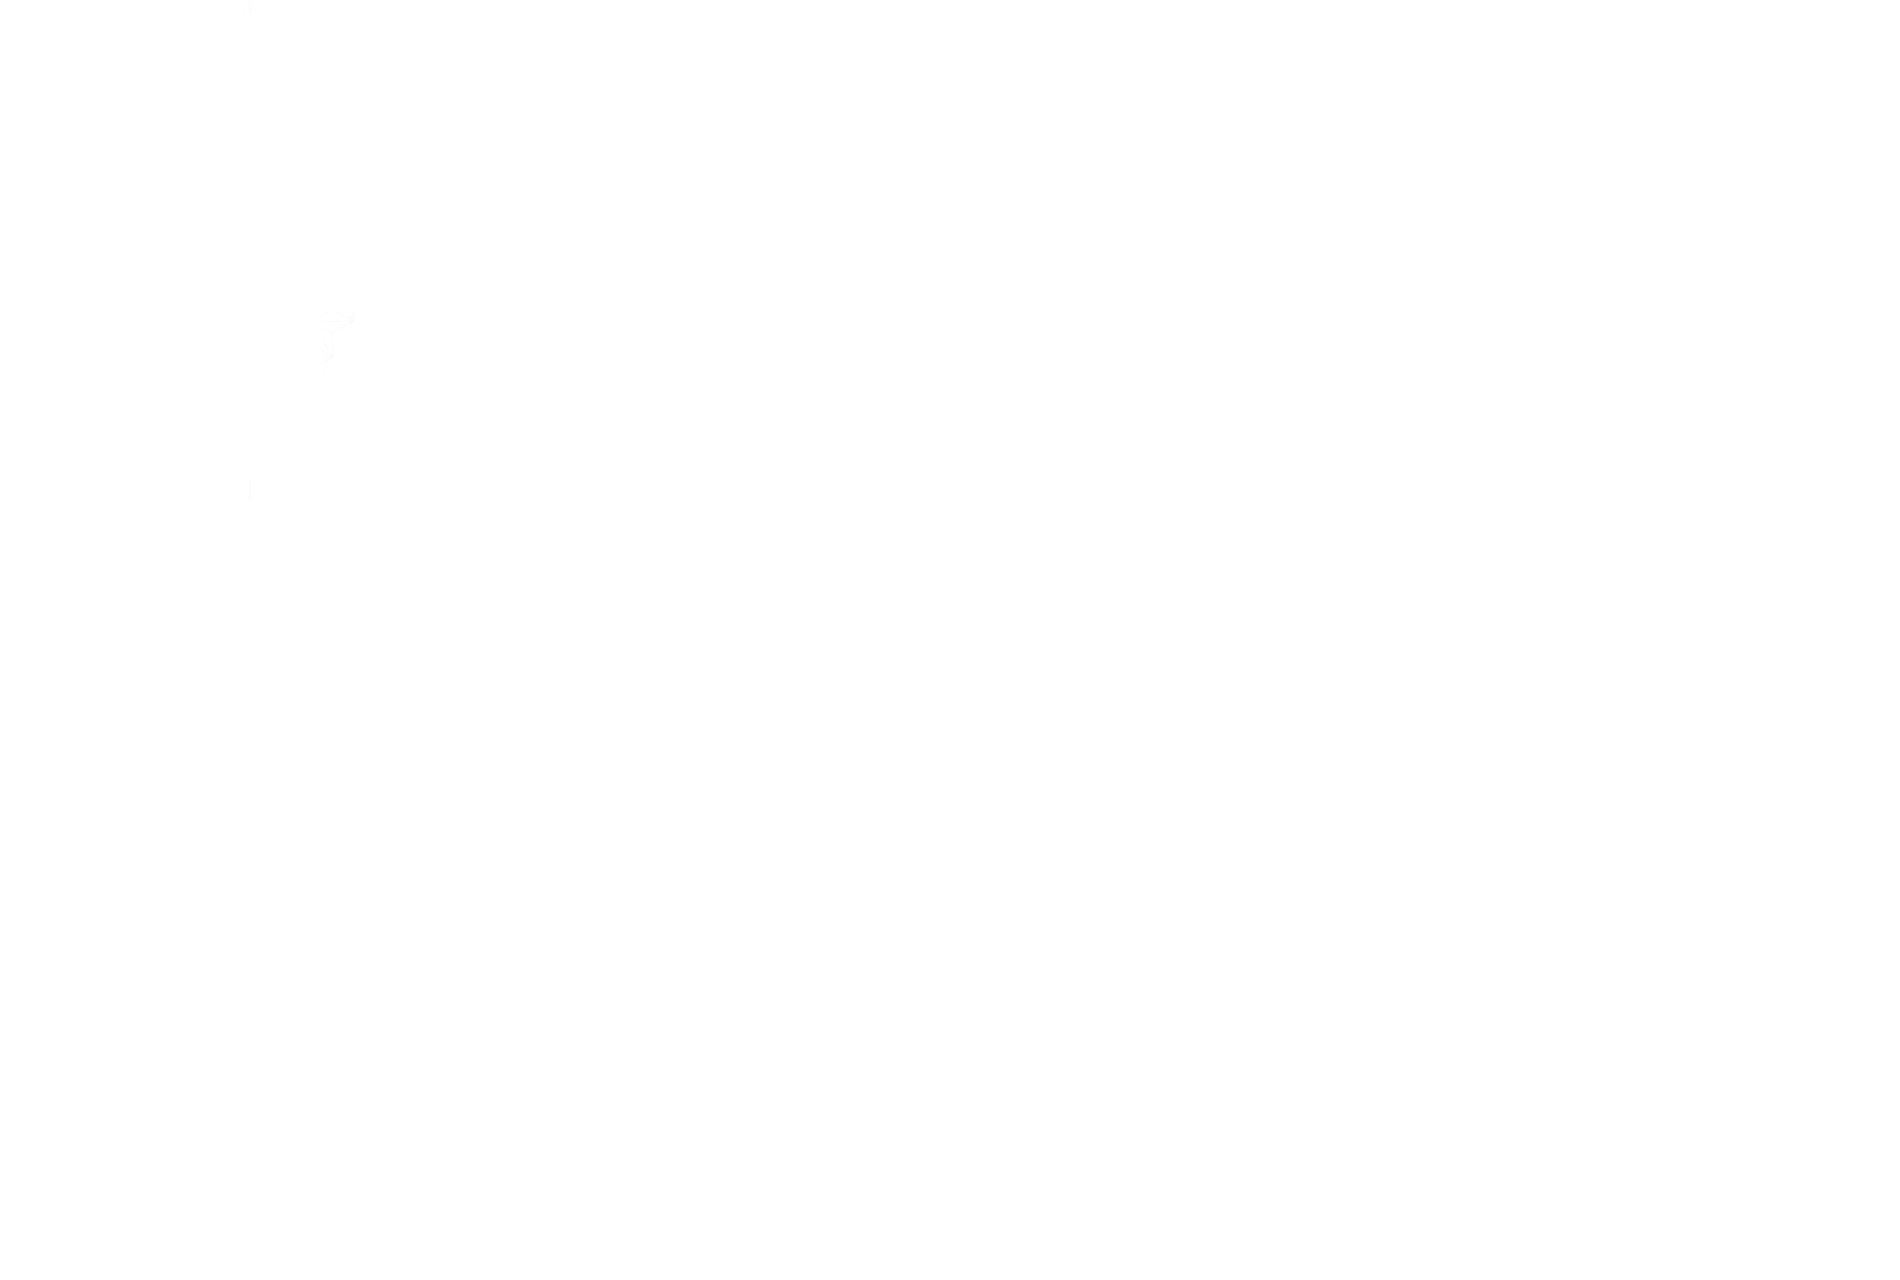
\includegraphics[width=\paperwidth,height=\paperheight]{images/bg}
		};
		\node[opacity=0.9] at (11.5,-2) {
			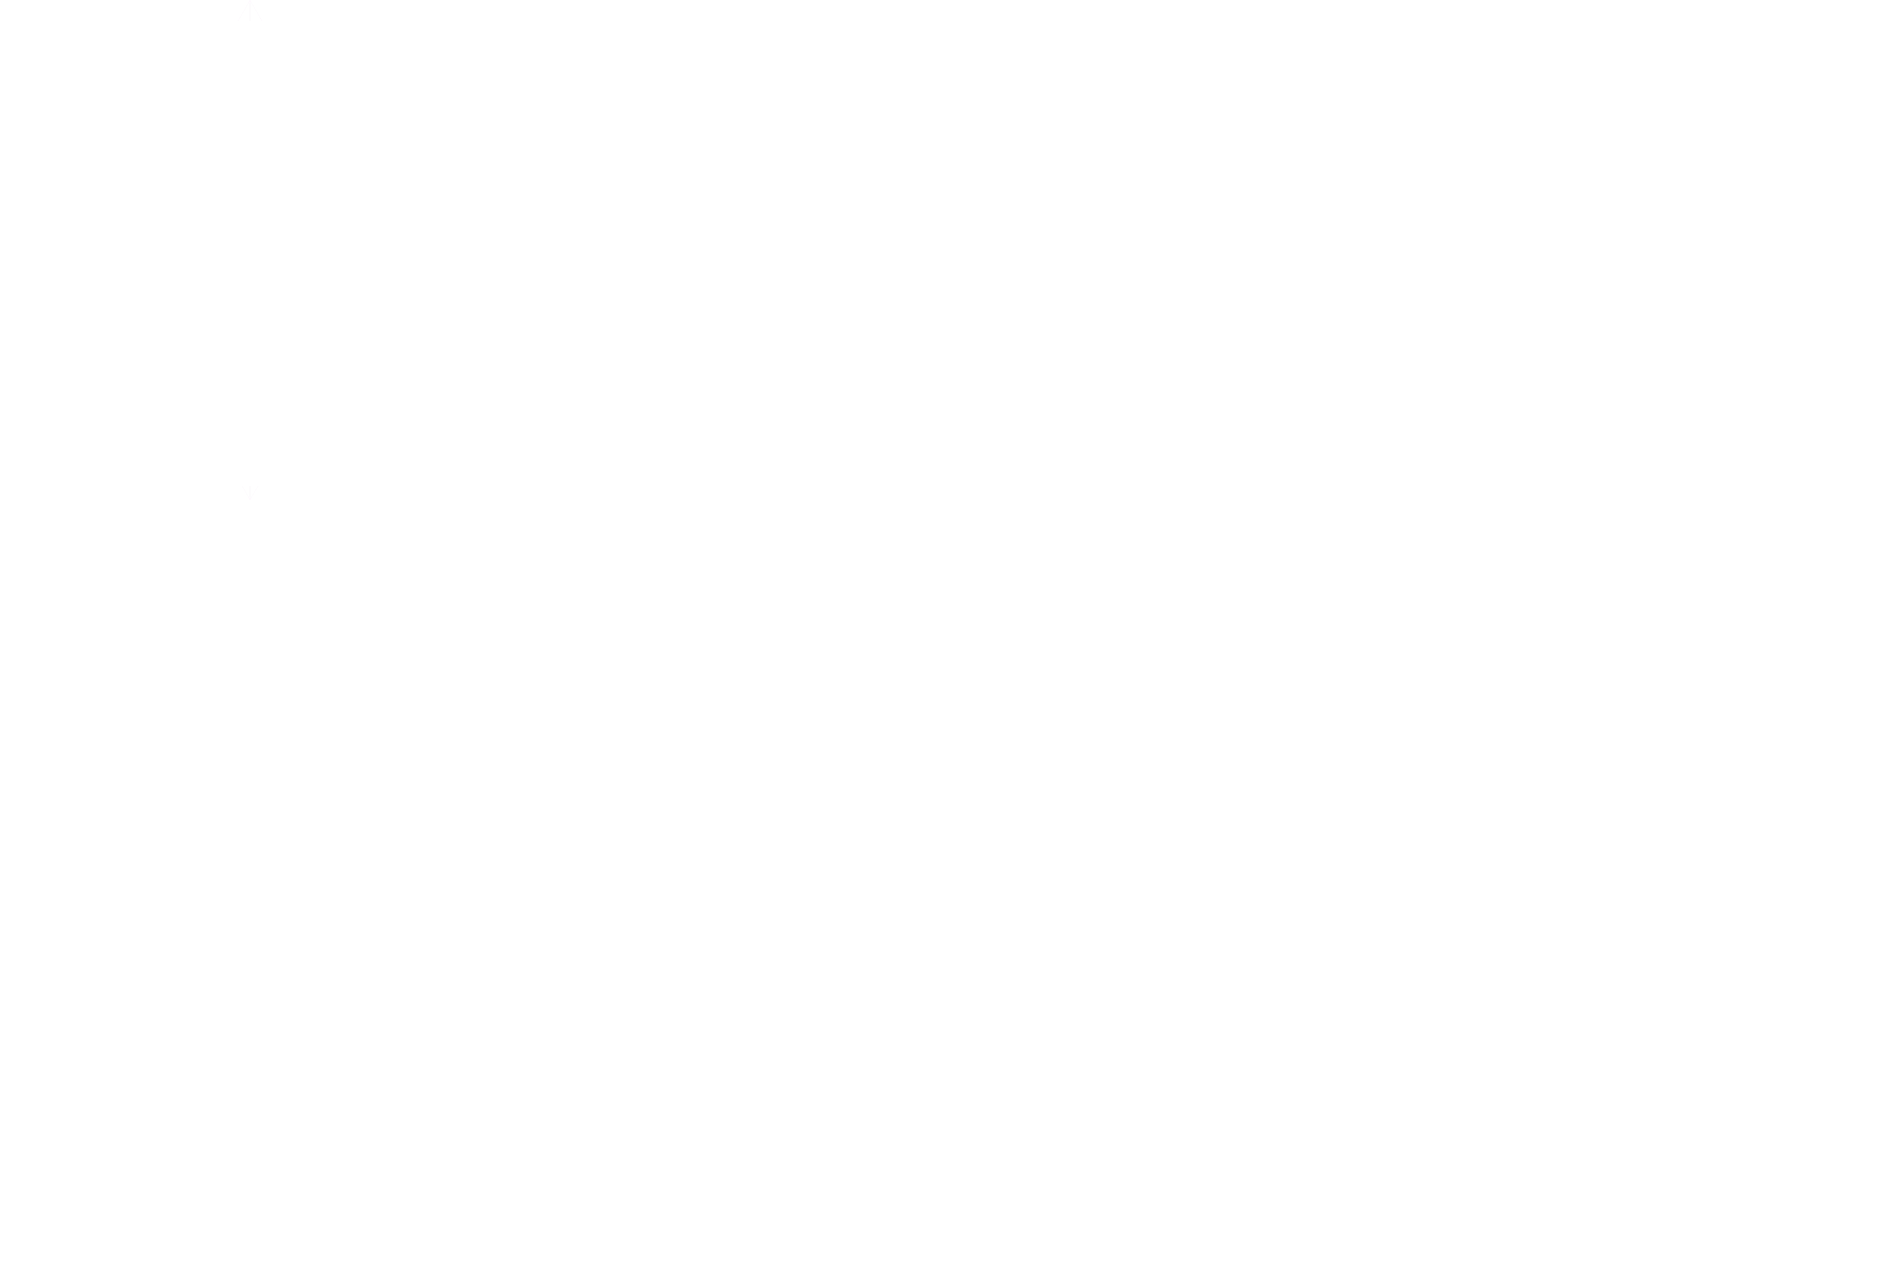
\includegraphics[keepaspectratio,scale=0.24]{images/title_logo}
		};
	\end{tikzpicture}
}
\setstretch{1.0}
\begin{frame}
\maketitle
\end{frame}
}

%\begin{frame}[fragile]
%\begin{center}
%\begin{tabular}{c}
%\begin{lstlisting}[basicstyle=\tiny,escapechar=!]
%Example code
%\end{lstlisting}
%\end{tabular}
%\end{center}
%\end{frame}

\begin{frame}[fragile]
\begin{center}
\begin{figure}
	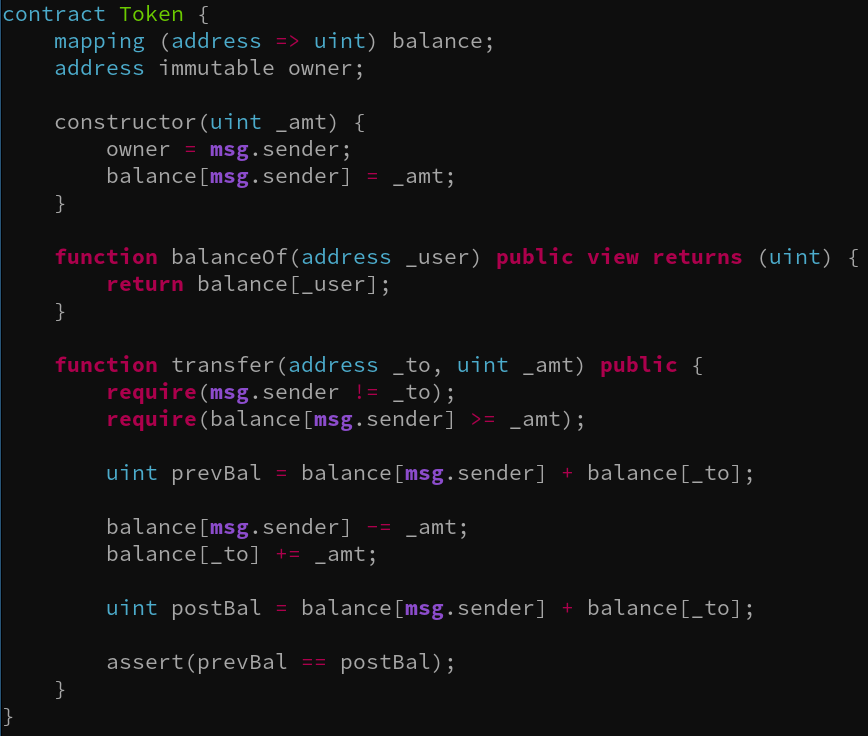
\includegraphics[scale=0.3]{images/token_pass}
\end{figure}
\end{center}
\end{frame}

\begin{frame}[fragile]
\begin{center}
\begin{figure}
	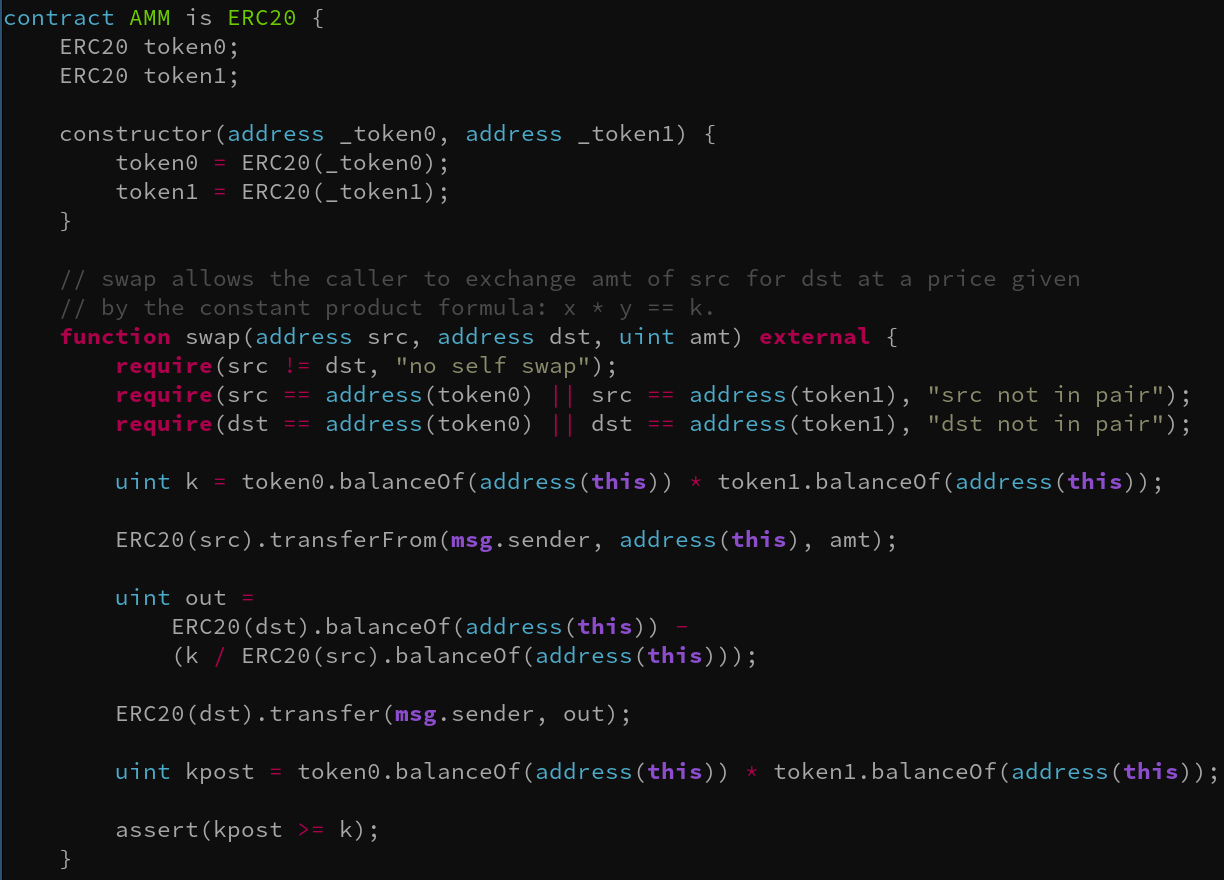
\includegraphics[scale=0.25]{images/amm_fail}
\end{figure}
\end{center}
\end{frame}

\begin{frame}[fragile]
\begin{center}
\begin{figure}
	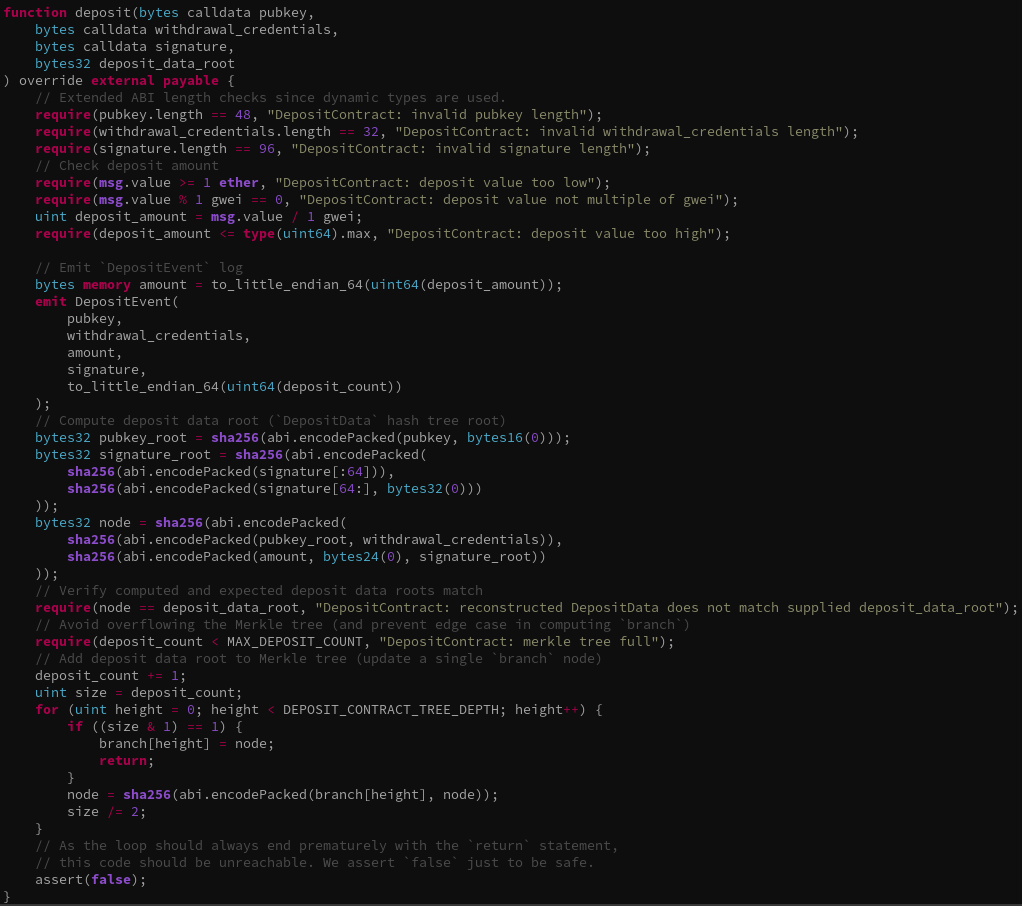
\includegraphics[scale=0.25]{images/deposit_pass}
\end{figure}
\end{center}
\end{frame}

\begin{frame}[fragile]
\begin{center}
\begin{figure}
	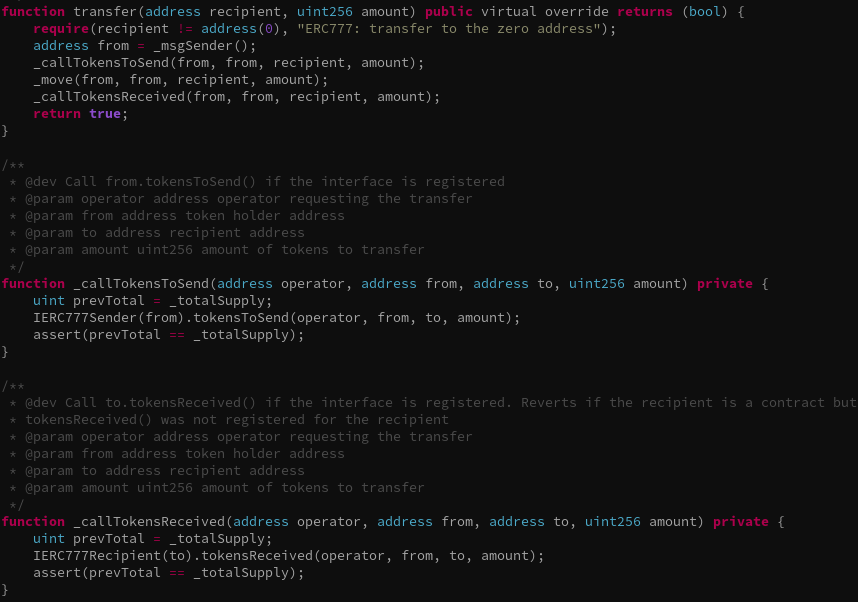
\includegraphics[scale=0.35]{images/erc777_fail}
\end{figure}
\end{center}
\end{frame}

\begin{frame}[fragile]
\begin{center}
\begin{itemize}
\item Mythril - symbolic execution
\item hevm - symbolic execution, invariant fuzzing
\item Echidna - invariant fuzzing
\item SMTChecker - model checking
\item solc-verify - model checking
\item VeriSmart - model checking
\end{itemize}
Tools that claim to try to prove/break properties automatically and are publicly available.
\end{center}
\end{frame}

\begin{frame}[fragile]
\begin{center}
Which tool can either {\color{green}{prove correctness}} or {\color{red}{find bugs}} in all the examples?
\end{center}
\end{frame}

\begin{frame}[fragile]
\begin{center}
None
\end{center}
\end{frame}

\begin{frame}[fragile]
\begin{center}
Automated formal verification is undecidable
\end{center}
\end{frame}

\begin{frame}[fragile]
Target Solidity\\
Cons
\begin{itemize}
\item A lot to encode: high level features, various data types, pointers, inheritance.
\item Results rely on compiler correctness.
\end{itemize}
Pros\\
\begin{itemize}
\item Gives more structure information, for example, loops, external calls, functions.
\item Can try harder problems, involving loop/contract invariants.
\end{itemize}
Model checking: SMTChecker, solc-verify, VeriSmart
\end{frame}

\begin{frame}[fragile]
Target EVM bytecode\\
Cons
\begin{itemize}
\item Not a lot of structure.
\item Hard to track storage, external calls, functions.
\item Needs to verify ABI encoding/decoding.
\end{itemize}
Pros\\
\begin{itemize}
\item Easier to encode.
\item Results are closer to the deployed object.
\end{itemize}
Symbolic execution and fuzzing: Mythril, hevm, Echidna
\end{frame}

\begin{frame}[fragile]
Experiment:
\begin{center}
Use each tool on each example, first automatically then tweaking parameters and writing specs taylored to the tool.
\end{center}
\end{frame}

\begin{frame}[fragile]
\begin{center}
Prove functional correctness of transfer function
\begin{figure}
	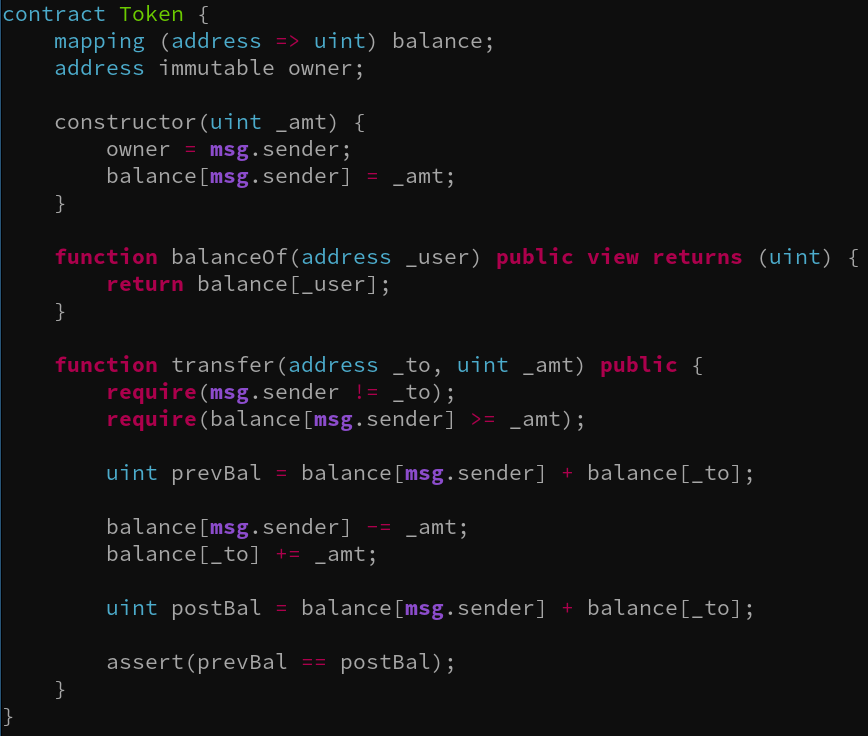
\includegraphics[scale=0.25]{images/token_pass}
\end{figure}
\end{center}
\end{frame}

\begin{frame}[fragile]
\begin{center}
Prove functional correctness of transfer function
\begin{itemize}
\item Mythril - OK
\item hevm - OK
\item Echidna - OK (no bugs found)
\item SMTChecker - OK
\item solc-verify - OK
\item VeriSmart - OK
\end{itemize}
\end{center}
\end{frame}

\begin{frame}[fragile]
\begin{center}
Find bug in buggy transfer function
\begin{figure}
	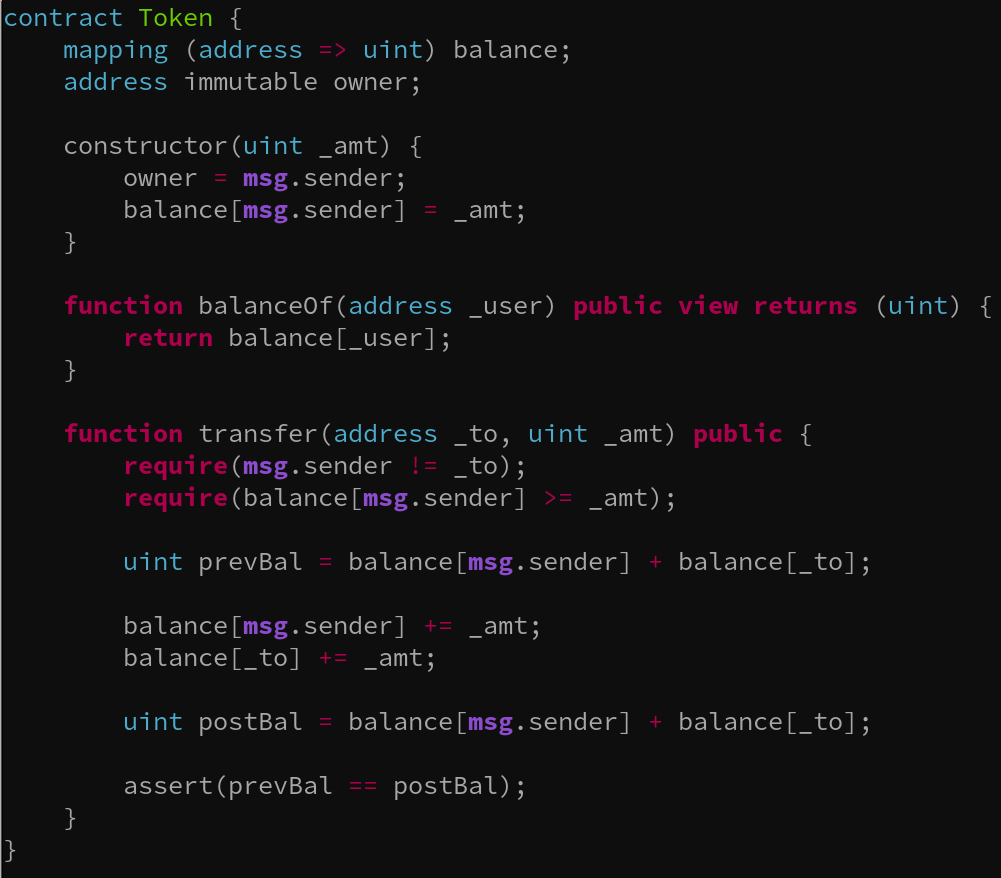
\includegraphics[scale=0.23]{images/token_fail}
\end{figure}
\end{center}
\end{frame}

\begin{frame}[fragile]
\begin{center}
Find bug in buggy transfer function
\begin{itemize}
\item Mythril - OK, with counterexample
\item hevm - OK, with counterexample
\item Echidna - OK, with counterexample
\item SMTChecker - OK, with counterexample
\item solc-verify - OK, no counterexample
\item VeriSmart - No
\end{itemize}
\end{center}
\end{frame}

\begin{frame}[fragile]
\begin{center}
AMM swap functional correctness (?)
\begin{figure}
	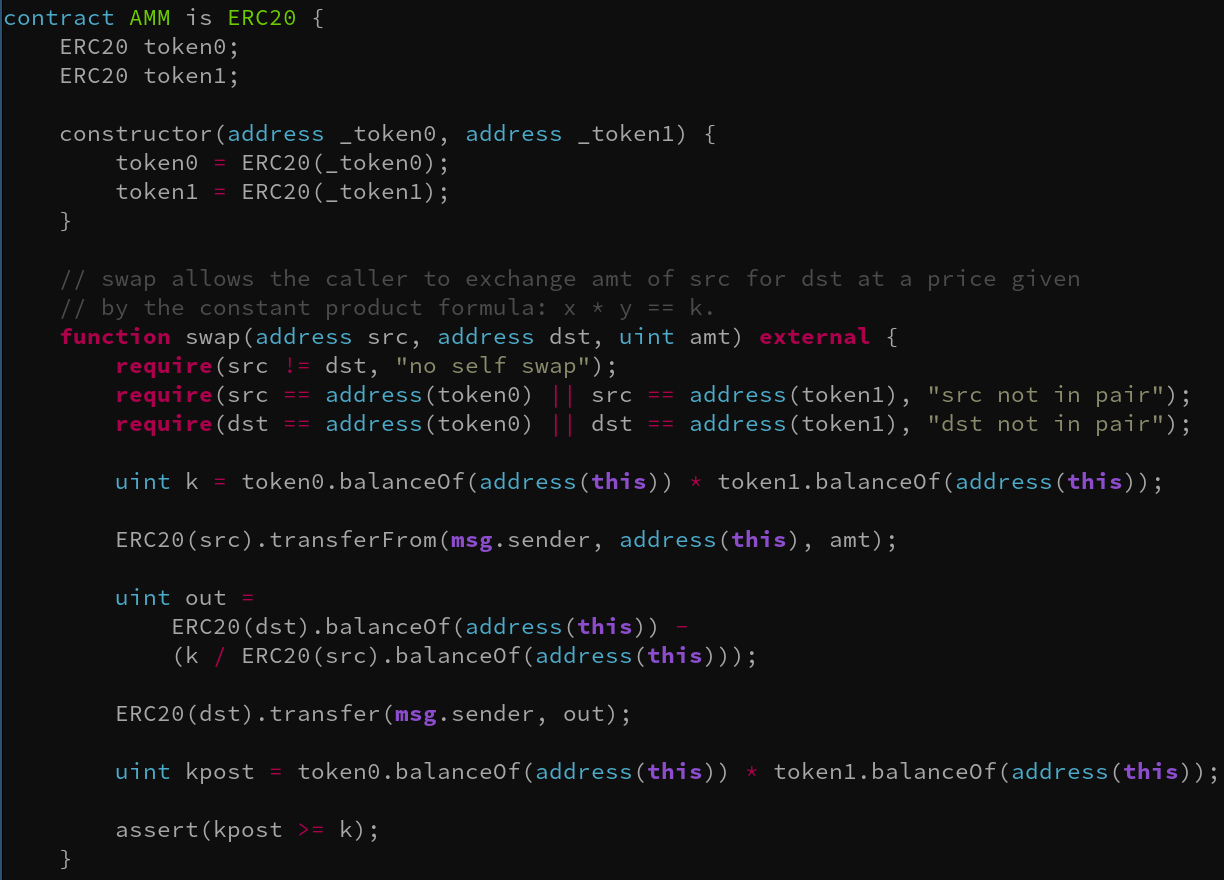
\includegraphics[scale=0.23]{images/amm_fail}
\end{figure}
\end{center}
\end{frame}

\begin{frame}[fragile]
\begin{center}
AMM swap functional correctness (?)\\
Symbolic execution and model checking tools could not prove/disprove the assertion
\end{center}
\end{frame}

\begin{frame}[fragile]
\begin{center}
AMM swap functional correctness (?)\\
Fuzzing?\\
\begin{figure}
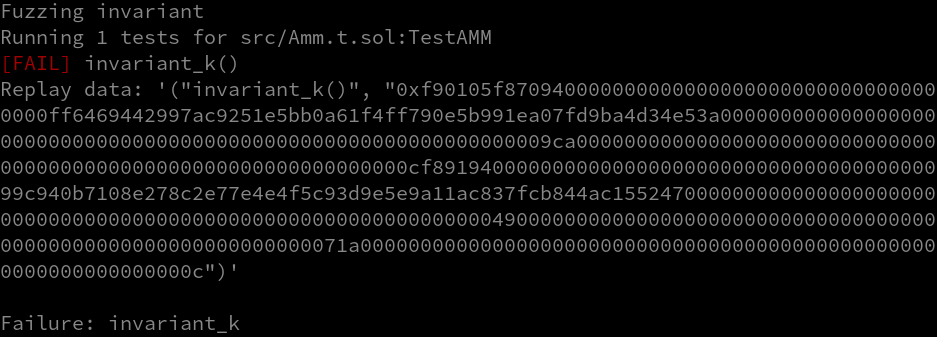
\includegraphics[scale=0.2]{images/amm_fail_hevm_run}
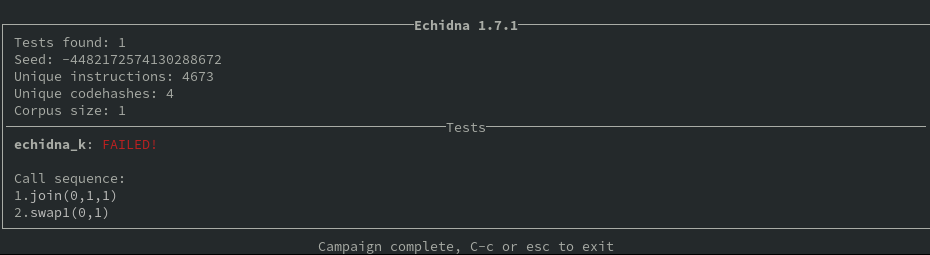
\includegraphics[scale=0.2]{images/amm_fail_echidna_run}
\end{figure}
\end{center}
\end{frame}

\begin{frame}[fragile]
\begin{center}
AMM swap functional correctness\\
Fuzzing with hevm
\begin{figure}
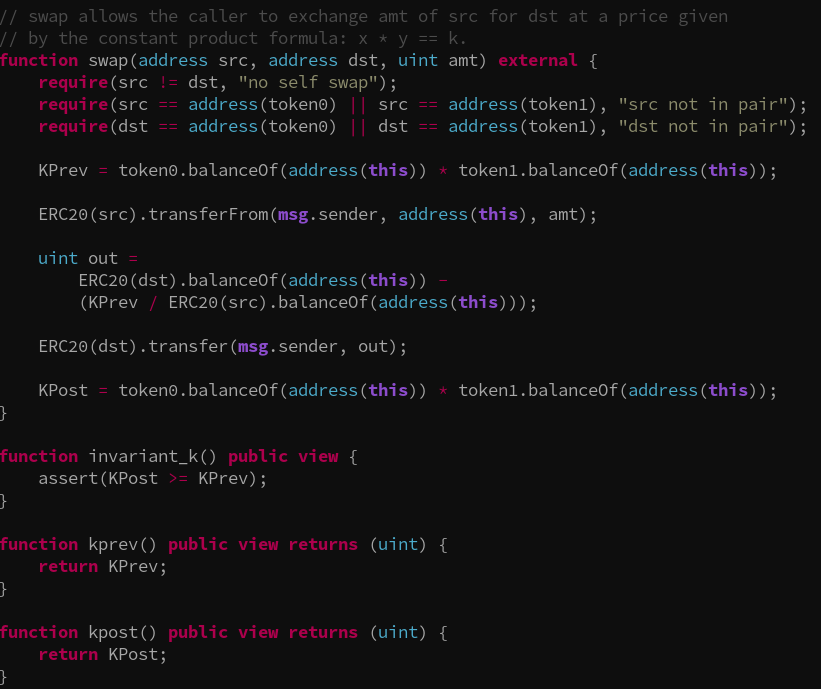
\includegraphics[scale=0.2]{images/amm_fail_hevm_code}
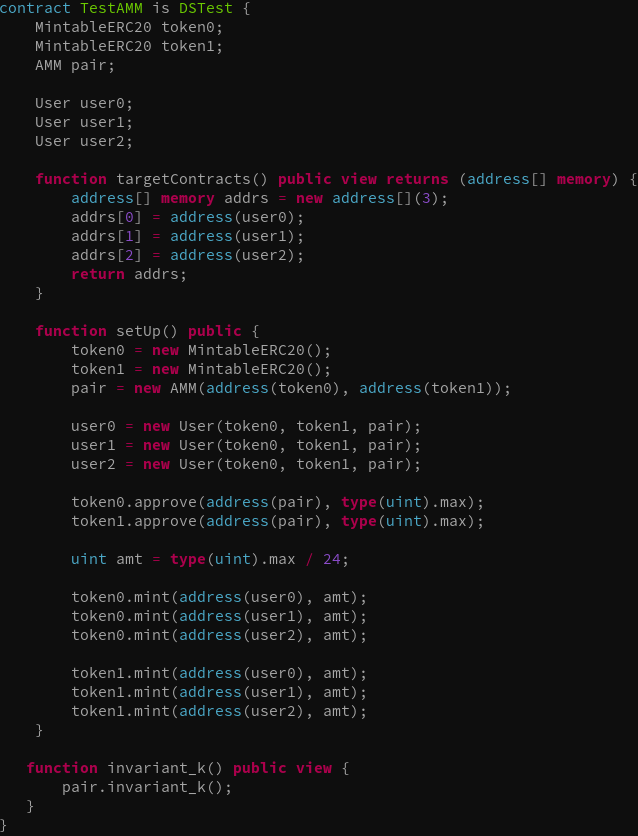
\includegraphics[scale=0.2]{images/amm_fail_hevm_code_test}
\end{figure}
\end{center}
\end{frame}

\begin{frame}[fragile]
\begin{center}
AMM swap functional correctness\\
Fuzzing with Echidna
\begin{figure}
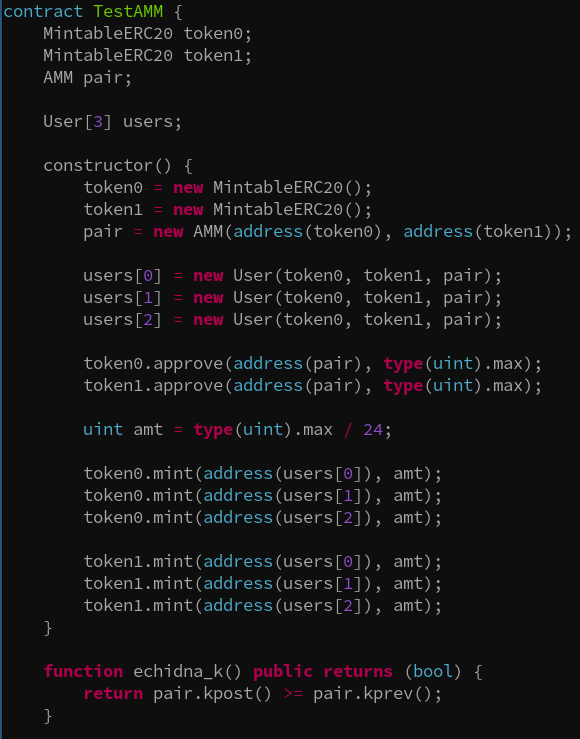
\includegraphics[scale=0.2]{images/amm_fail_echidna_code_test}
\end{figure}
\end{center}
\end{frame}

\begin{frame}[fragile]
\begin{center}
AMM swap functional correctness
\begin{figure}
	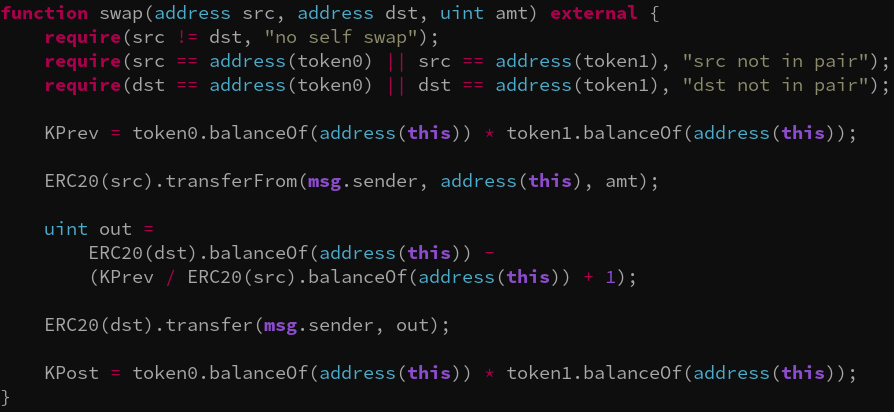
\includegraphics[scale=0.35]{images/amm_pass}
\end{figure}
\end{center}
\end{frame}

\begin{frame}[fragile]
\begin{center}
Model checkers still cannot prove correctness, but fuzzers could not find any other problems.
\begin{figure}
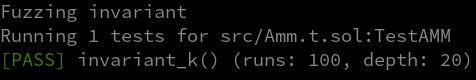
\includegraphics[scale=0.35]{images/amm_pass_hevm_run}
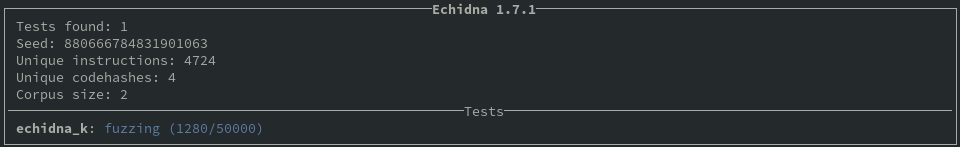
\includegraphics[scale=0.35]{images/amm_pass_echidna_run}
\end{figure}
\end{center}
\end{frame}

\begin{frame}[fragile]
\begin{center}
Prove function correctness of deposit
\begin{figure}
	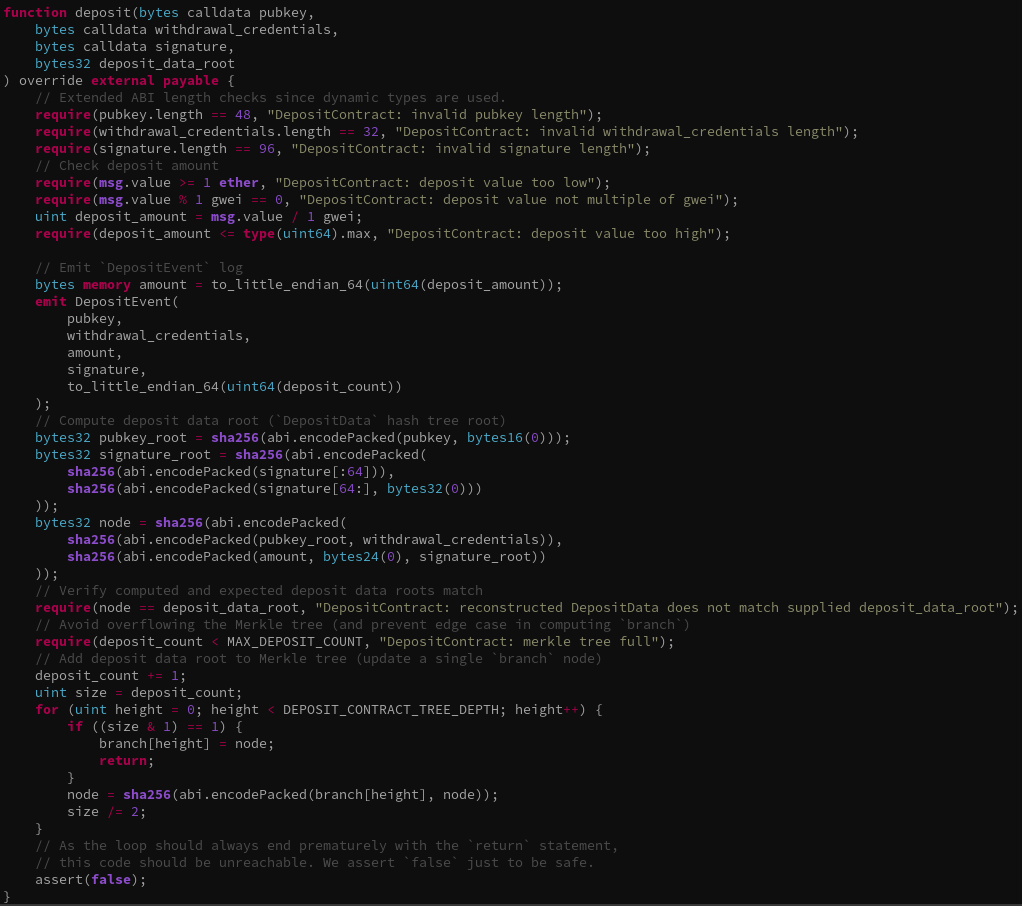
\includegraphics[scale=0.25]{images/deposit_pass}
\end{figure}
\end{center}
\end{frame}

\begin{frame}[fragile]
\begin{center}
Prove function correctness of deposit:\\
No tool could prove that the assertion is not reachable automatically.\\
\end{center}
\end{frame}

\begin{frame}[fragile]
\begin{center}
Modified version for hevm
\begin{figure}
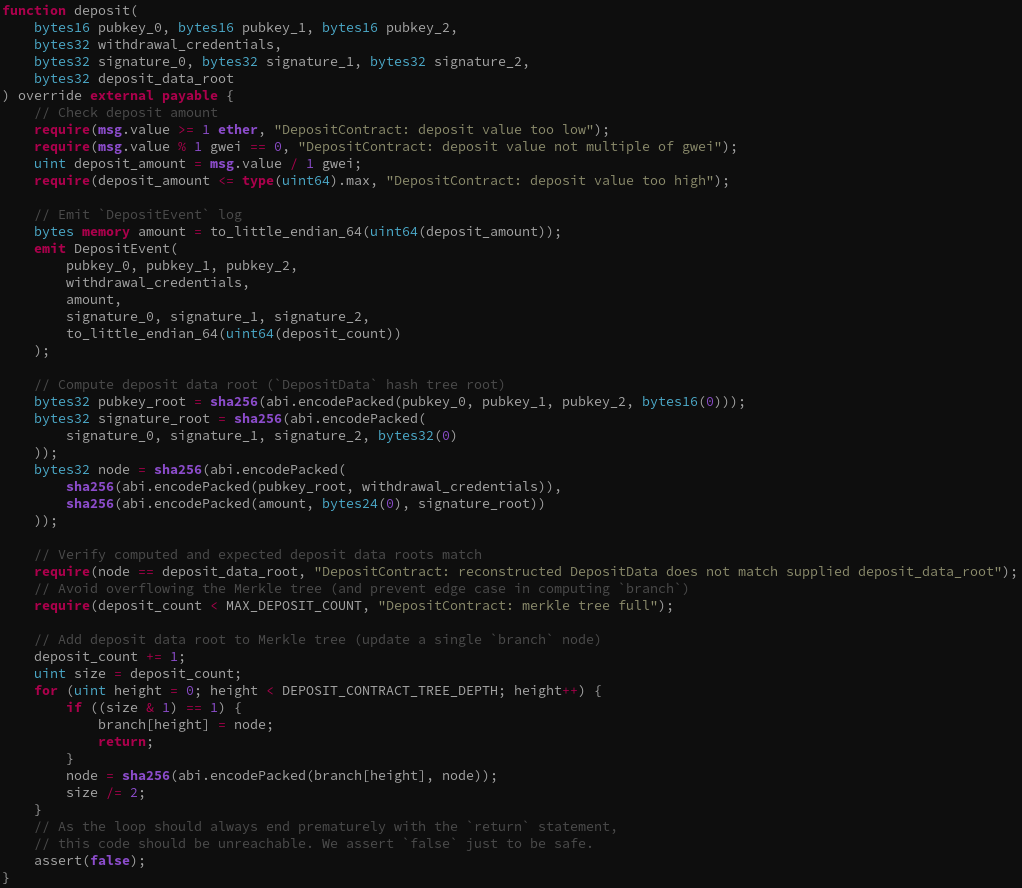
\includegraphics[scale=0.22]{images/deposit_hevm_code}
\end{figure}
\end{center}
\end{frame}

\begin{frame}[fragile]
\begin{center}
hevm results
\begin{figure}
	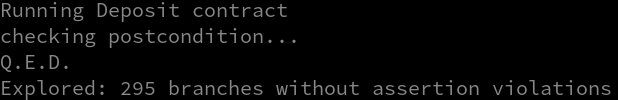
\includegraphics[scale=0.35]{images/deposit_hevm_run}
\end{figure}
\end{center}
\end{frame}

\begin{frame}[fragile]
\begin{center}
Modified version for SMTChecker
\begin{figure}
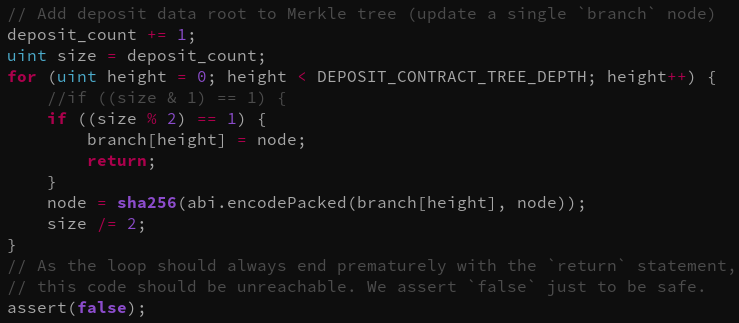
\includegraphics[scale=0.25]{images/deposit_smtchecker_code}
\end{figure}
+ use non default Horn solver Eldarica via solc-js' SMT callback\\
+ use Eldarica's \emph{abstract:off} option
\end{center}
\end{frame}

\begin{frame}[fragile]
\begin{center}
SMTChecker's inductive invariant for the loop before the assertion
\begin{figure}

\includegraphics[scale=0.2]{images/deposit_pass_smtchecker_proof}
\end{figure}
\end{center}
\end{frame}

\begin{frame}[fragile]
\begin{center}
Prove ERC777 property in the presence of external calls
\begin{figure}
	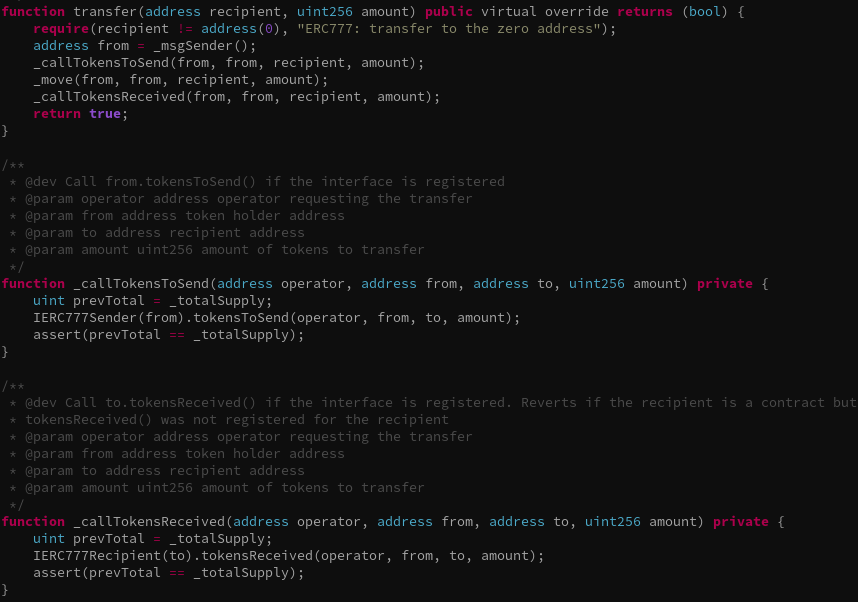
\includegraphics[scale=0.3]{images/erc777_fail}
\end{figure}
\end{center}
\end{frame}

\begin{frame}[fragile]
\begin{center}
SMTChecker says that the property does not hold
\begin{figure}
	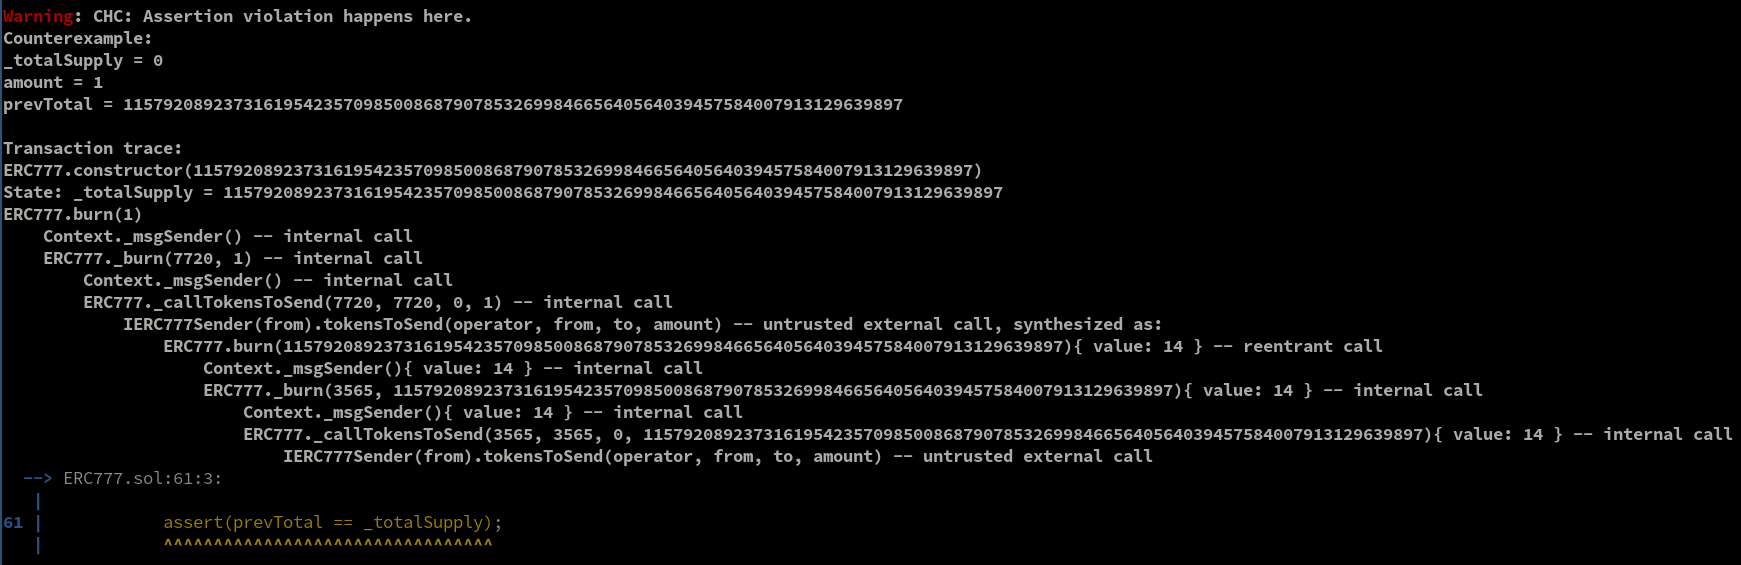
\includegraphics[scale=0.23]{images/erc777_fail_smtchecker_cex}
\end{figure}
- Remove strings (hard for counterexamples)
\end{center}
\end{frame}

\begin{frame}[fragile]
\begin{center}
Let's test that
\begin{figure}
	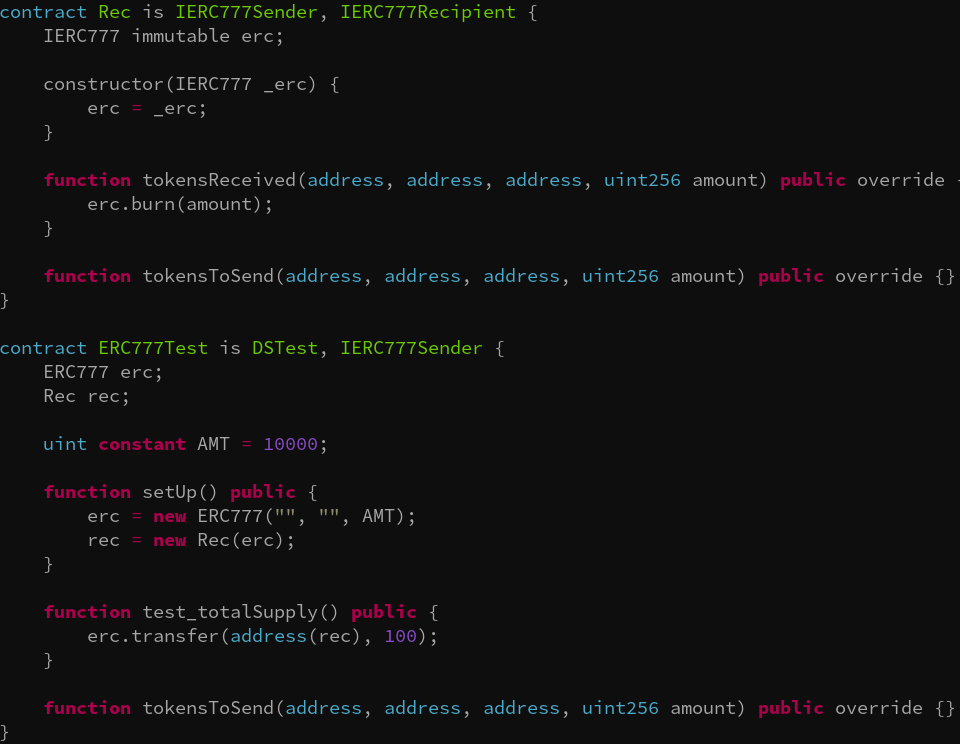
\includegraphics[scale=0.25]{images/erc777_fail_hevm_test_code}
\end{figure}
\end{center}
\end{frame}

\begin{frame}[fragile]
\begin{center}
Property is indeed broken
\begin{figure}
	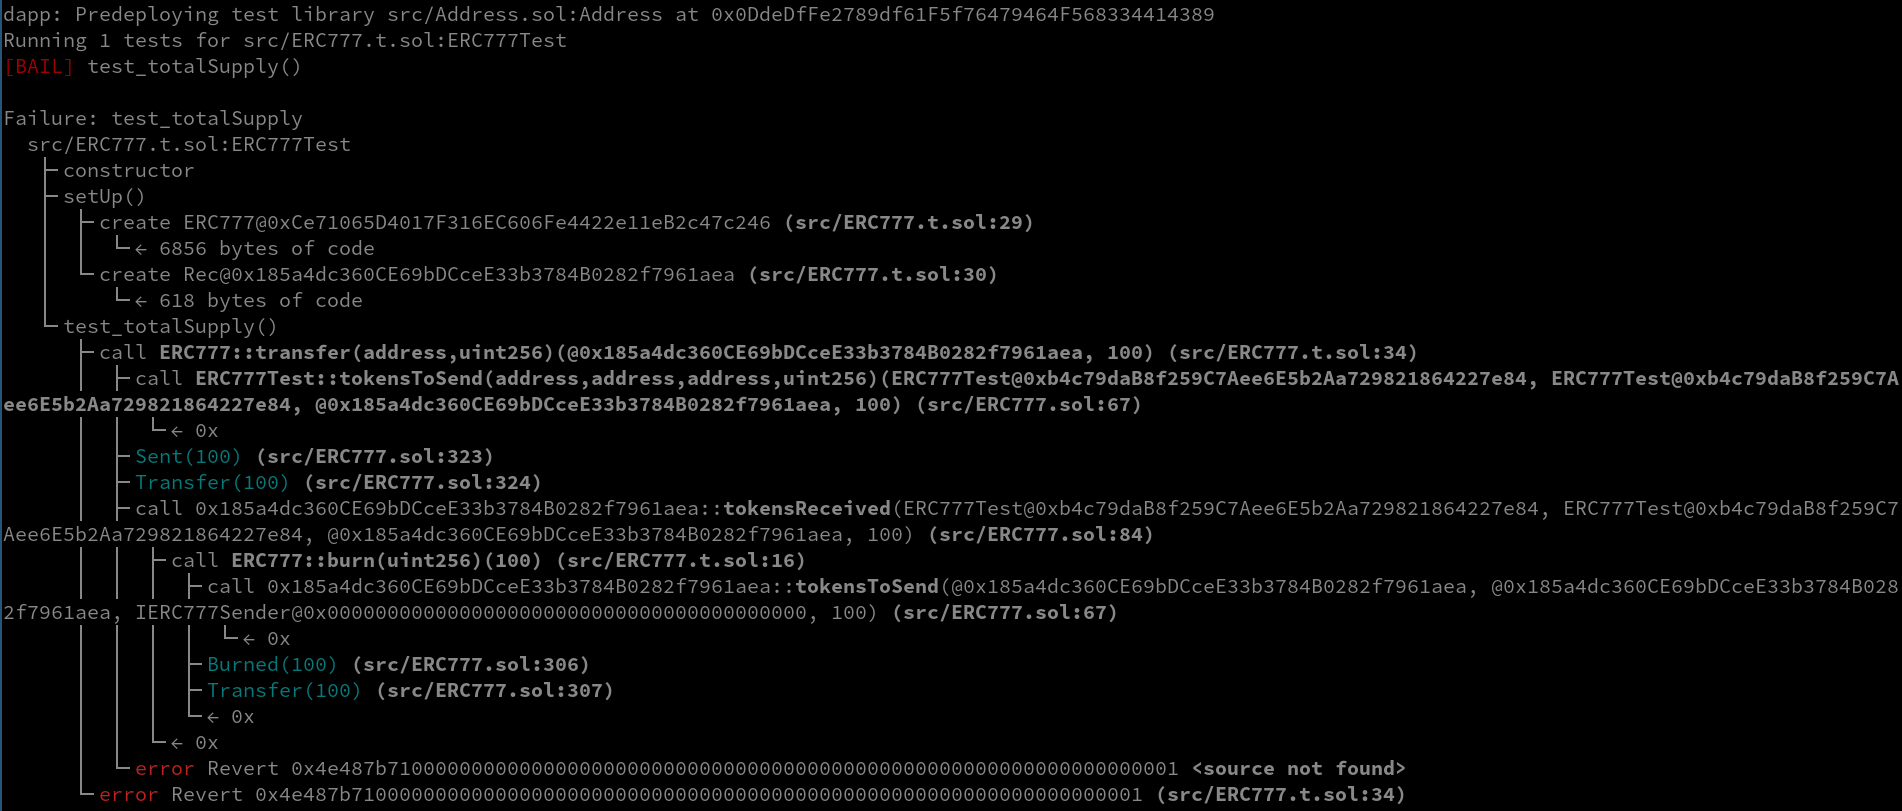
\includegraphics[scale=0.2]{images/erc777_fail_hevm_test}
\end{figure}
\end{center}
\end{frame}

\begin{frame}[fragile]
\begin{center}
We can forbid reentrancy
\begin{figure}
	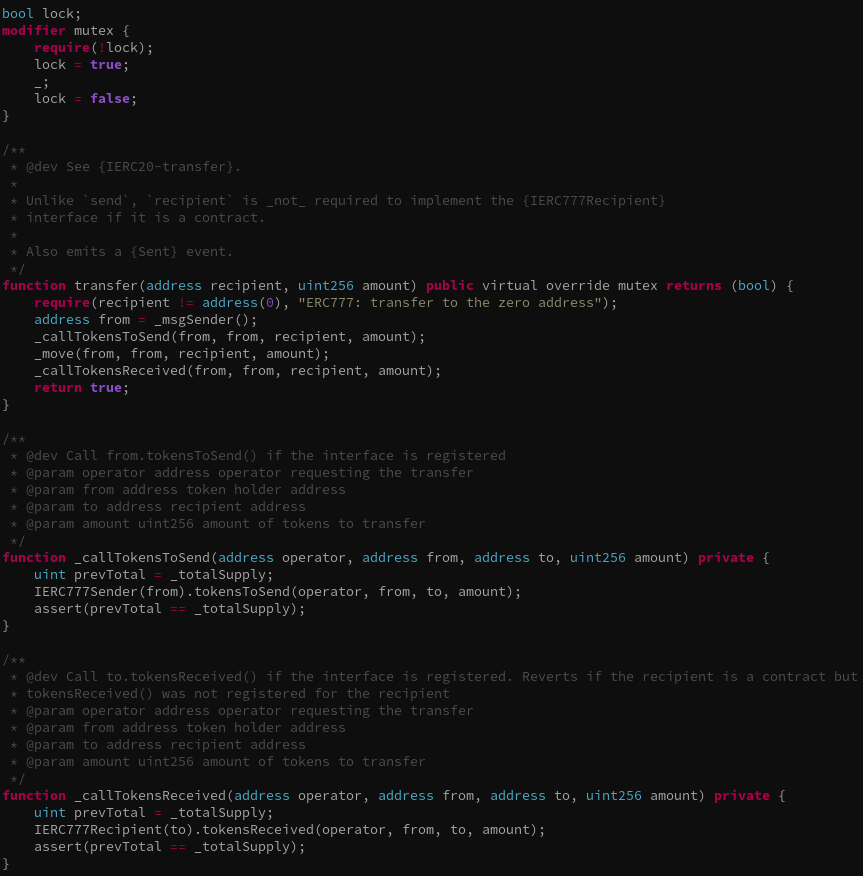
\includegraphics[scale=0.23]{images/erc777_pass_mutex_smtchecker}
\end{figure}
\end{center}
\end{frame}

\begin{frame}[fragile]
\begin{center}
Are we safe now? Reentrancy guard blocks the tx before the assertion failure
\begin{figure}
	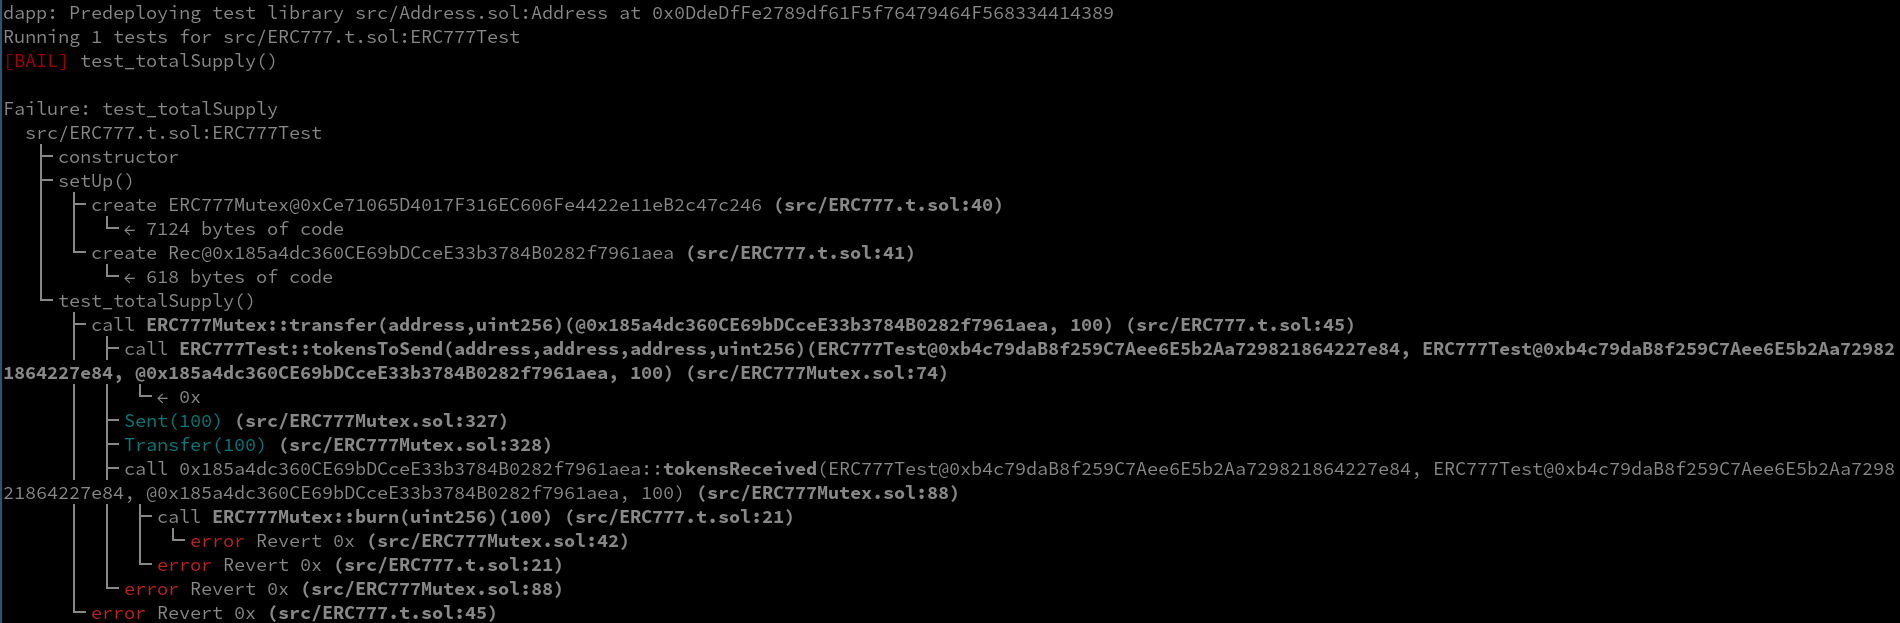
\includegraphics[scale=0.2]{images/erc777_fail_hevm_test_mutex}
\end{figure}
\end{center}
\end{frame}

\begin{frame}[fragile]
\begin{center}
SMTChecker proves that now the assertions are safe
\begin{figure}
	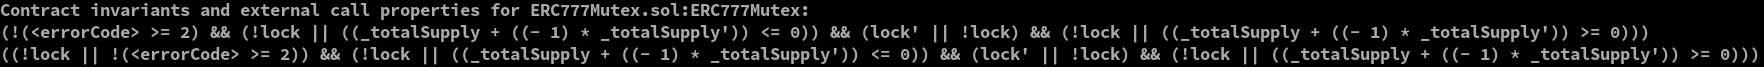
\includegraphics[scale=0.23]{images/erc777_pass_smtchecker_invariants}
\end{figure}
$lock \implies (\_totalSupply = \_totalSupply')$
\end{center}
\end{frame}

\begin{frame}[fragile]
\begin{center}
SMTChecker internals
\begin{figure}
	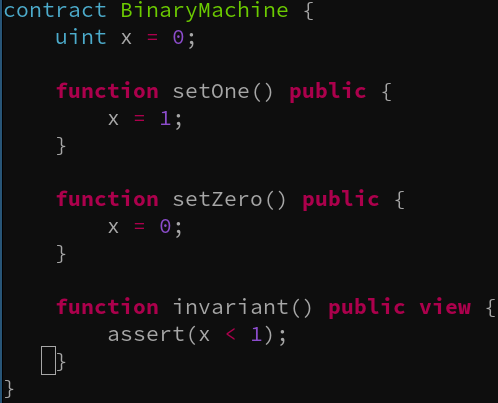
\includegraphics[scale=0.4]{images/binary_machine_code}
\end{figure}
\end{center}
\end{frame}

\begin{frame}[fragile]
{\small
\begin{align*}
error = 0 \land x = 0  & \implies constructor(error, x) \\
error = 0 \land x = x' & \implies setOneEntry(error, x, x') \\
setOneEntry(error, x, x') & \implies setOneSummary(error, x, 1) \\
error = 0 \land x = x' & \implies setZeroEntry(error, x, x') \\
setZeroEntry(error, x, x') & \implies setZeroSummary(error, x, 0) \\
error = 0 \land x = x' & \implies invariantEntry(error, x, x') \\
invariantEntry(error, x, x') \land x \ge 2 \land errorCode = 1 & \implies invariantSummary(errorCode, x, x') \\
invariantEntry(error, x, x') \land x < 2 & \implies invariantSummary(error, x, 1) \\
\end{align*}
}%
\end{frame}

\begin{frame}[fragile]
{\small
\begin{align*}
error = 0 \land	constructor(error, x) & \implies interface(x) \\
interface(x) \land setOneSummary(error, x, x') \land error = 0 & \implies interface(x') \\
interface(x) \land setOneSummary(error, x, x') \land error > 0 & \implies errorTarget(error) \\
interface(x) \land setZeroSummary(error, x, x') \land error = 0 & \implies interface(x') \\
interface(x) \land setZeroSummary(error, x, x') \land error > 0 & \implies errorTarget(error) \\
interface(x) \land invariantSummary(error, x, x') \land error = 0 & \implies interface(x') \\
interface(x) \land invariantSummary(error, x, x') \land error > 0 & \implies errorTarget(error) \\
\end{align*}
}%
\end{frame}

\begin{frame}[fragile]
\begin{center}
Counterexample graph
\begin{figure}
	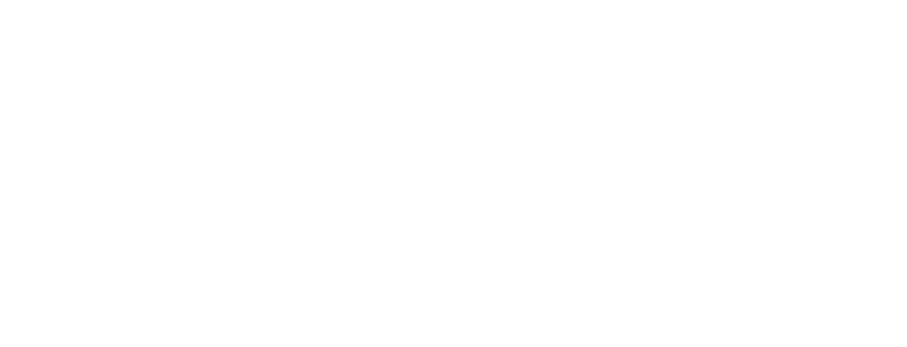
\includegraphics[scale=0.4]{images/binary_machine_cex_graph}
\end{figure}
\end{center}
\end{frame}

\begin{frame}[fragile]
\begin{center}
Correct code
\begin{figure}
	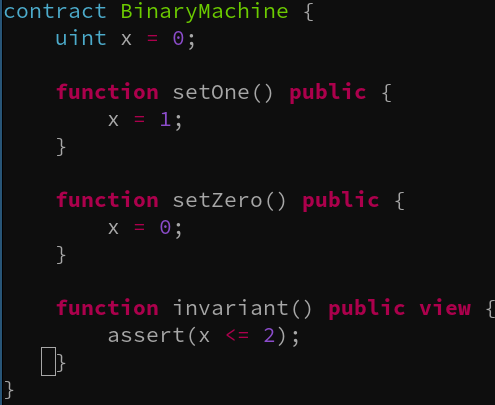
\includegraphics[scale=0.4]{images/binary_machine_code_pass}
\end{figure}
\end{center}
\end{frame}

\begin{frame}[fragile]
\begin{center}
Inductive invariants\\
\;\\
$interface(e, x) = x < 2$\\
$invariantSummary(e, x, x') = x' = 0 \lor x' = 1$\\
$constructorSummary(e, x) = e = 0 \land x' = 0$\\
$setOneSummary(e, x, x') = e = 0 \land x' = 1$\\
$setZeroSummary(e, x, x') = e = 0 \land x' = 0$\\
\end{center}
\end{frame}

\begin{frame}[fragile]
\begin{center}
SMTChecker internals - External calls
\begin{figure}
	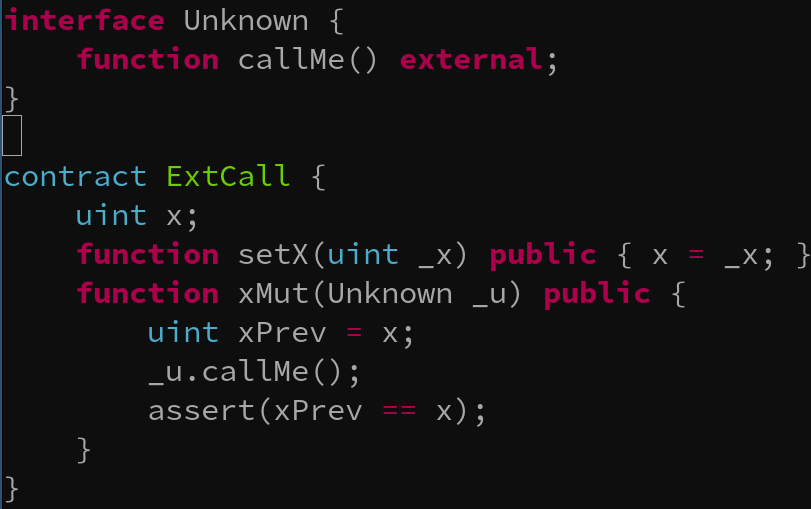
\includegraphics[scale=0.3]{images/extcall_fail_code}
\end{figure}
\end{center}
\end{frame}

\begin{frame}[fragile]
New rules help with synthesis of externally called unknown functions
{\small
\begin{align*}
error = 0 \implies nondetInterface(error, x, x') \\
error = 0 \land	nondetInterface(error, x, x') \land setX(error', x', x'') \implies nondetInterface(error', x, x'') \\
error = 0 \land	nondetInterface(error, x, x') \land xMut(error', x', x'') \implies nondetInterface(error', x, x'') \\
\end{align*}
}%
\end{frame}

\begin{frame}[fragile]
\begin{center}
Counterexample graph synthesizing external calls
\begin{figure}
	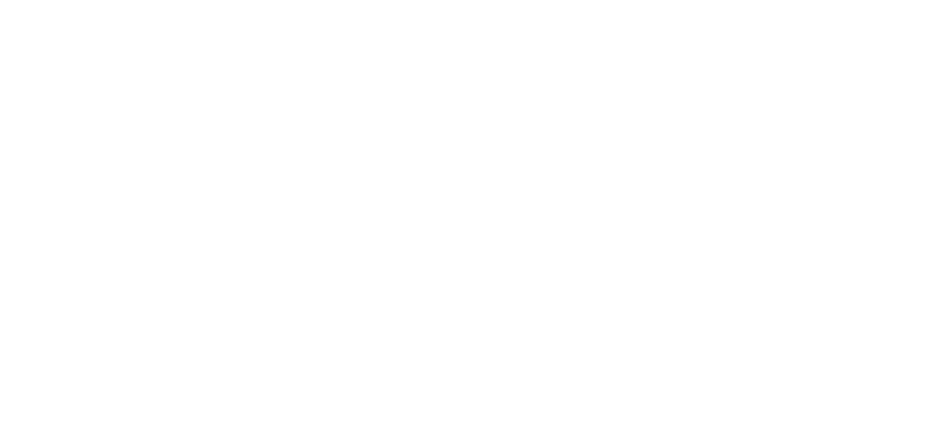
\includegraphics[scale=0.4]{images/extcall_fail_cex_graph}
\end{figure}
\end{center}
\end{frame}

\begin{frame}[fragile]
\begin{center}
SMTChecker internals - External calls
\begin{figure}
	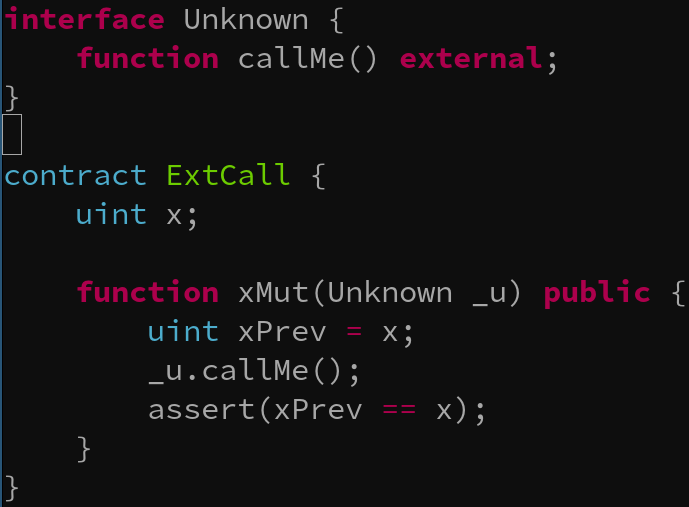
\includegraphics[scale=0.3]{images/extcall_pass_code}
\end{figure}
\end{center}
\end{frame}

\begin{frame}[fragile]
\begin{center}
Inductive invariants and external call properties\\
\;\\
$externalCallUnknown(e, x, x') = (x = 0 \implies e = 0) \land (x = 0 \implies x' = 0)$\\
$interface(x) = x = 0$
\end{center}
\end{frame}


\begin{frame}[fragile]
\begin{center}
hevm internals - Symbolic execution
\;\\
Execute EVM while building an AST for symbolic terms\\
Upon JUMPI, explore both paths add new constraint\\
Avoid infinite loops by `--max-iterations`\\
For all end states violating the property, check if constraints are satisfiable
\end{center}
\end{frame}

\begin{frame}[fragile]
\begin{center}
hevm internals - Symbolic ds-tests & rpc
\;\\
\begin{verbatim}
data StorageModel
  = ConcreteS    -- ^ Uses `Concrete` Storage. Reading / Writing from abstract
                 -- locations causes a runtime failure. Can be nicely combined with RPC.

  | SymbolicS    -- ^ Uses `Symbolic` Storage. Reading / Writing never reaches RPC,
                 -- but always done using an SMT array with no default value.

  | InitialS     -- ^ Uses `Symbolic` Storage. Reading / Writing never reaches RPC,
                 -- but always done using an SMT array with 0 as the default value.
\end{verbatim}
\end{center}
\end{frame}

\begin{frame}[fragile]
\begin{center}
hevm internals - Equivalence checking
\;\\
Make two copies of an abstract VM, differing only in the code of the current contract\\
Execute both symbolically and take all pairs of endstates\\
For every pair, check if both constraint sets are satisfiable and if results differ\\
If no such pair exists, the contracts are equivalent\\
\end{center}
\end{frame}

\begin{frame}[fragile]
\begin{center}
Conclusions
\begin{itemize}
\item Automated FV tools can be quite powerful but...
\item No automated tool will do the job everytime
\item FV is still an expert domain
\item Specific tool knowledge is required to extract full potential
\item Playing with the tool is essential to get good results
\end{itemize}
\end{center}
\end{frame}

\begin{frame}[standout,fragile]
\begin{center}
Thank you!
\end{center}
\end{frame}
 
\end{document}
